\clearpage{\pagestyle{empty}\cleardoublepage}
\chapter{Introduzione al fotovoltaico}
%
Per \emph{impianto fovoltaico} si intende un qualunque 
impianto di produzione di energia elettrica che sfrutti, ai fini 
di produzione della stessa, l'\emph{effetto fotovoltaico}.
%
Ne esistono due grandi tipologie: impianti \emph{a isola} (o \emph{stand alone}), 
e impianti \emph{grid connected}, ovvero connessi alla rete nazionale in 
corrente alternata.
%
Oggetto di questa tesi saranno solo questi ultimi, in quanto sono gli unici
di cui abbia senso monitorare e quantificare la produzione energetica; gli impianti 
a isola, infatti, non sono generalmente utilizzati per la produzione di grandi
quantit\`a d'energia, piuttosto trovano applicazione laddove \`e necessario
rendere un sistema elettricamente \emph{autosufficiente}, p.es. per la 
ricarica di dispositivi alimentati a batteria.
%

%
Iniziamo la panoramica sugli impianti fotovolatici partendo dal fenomeno
che sta alla base del loro funzionamento: l'effetto fotovoltaico.
%

%
\section{L'effetto fotovoltaico}
L'\emph{effetto fotovoltaico} consiste nel passaggio di elettroni 
dalla \emph{banda di valenza} alla \emph{banda di conduzione} di 
un materiale, a causa dell'assorbimento di \emph{fotoni}. 
%
Tale fenomeno viene sfruttato dai \emph{moduli (o celle) fotovoltaici}, 
come mostrato in figura \ref{effetto-fv} allo scopo di trasformare 
l'energia insita nella radiazione luminosa in energia elettrica.
%
\begin{figure}[!h]
\centering
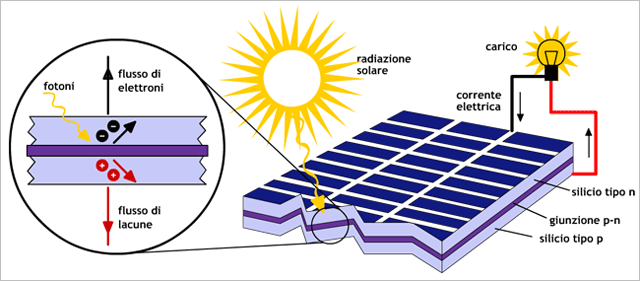
\includegraphics[width=350pt]{img/effetto-fovoltaico.png}
\caption{Effetto fotovoltaico}
\label{effetto-fv}
\end{figure}
%

%
\section{Architettura degli impianti grid-connected}
\subsection{I moduli fotovoltaici}
I moduli fotovoltaici sono gli elementi base di ogni impianto. 
Si tratta di dispositivi costituiti da \emph{fette} di materiale 
\emph{semiconduttore}, caratterizzato quindi da un \emph{band gap} 
di dimensioni tali per cui 
%
\begin{itemize}
\item a seguito dell'apporto energetico fornito dalla radiazione luminosa, 
      gli elettroni riescono a \emph{saltare} dalla banda di valenza a 
      quella di conduzione
      \footnote{ci\`o non sarebbe possibile in un \emph{isolante}}
%
\item gli elettroni che effettuano il \emph{salto} nella banda di conduzione 
      non vengono neutralizzati
      \footnote{come, invece, avverrebbe in un \emph{conduttore}}
\end{itemize}
%
La presenza di \emph{portatori di carica} nella banda di conduzione 
fa si che il modulo fotovoltaico, una volta connesso ad un conduttore 
esterno, si comporti come un \emph{generatore di corrente}\cite{bellini09}.
%
\begin{figure}[!h]
\centering
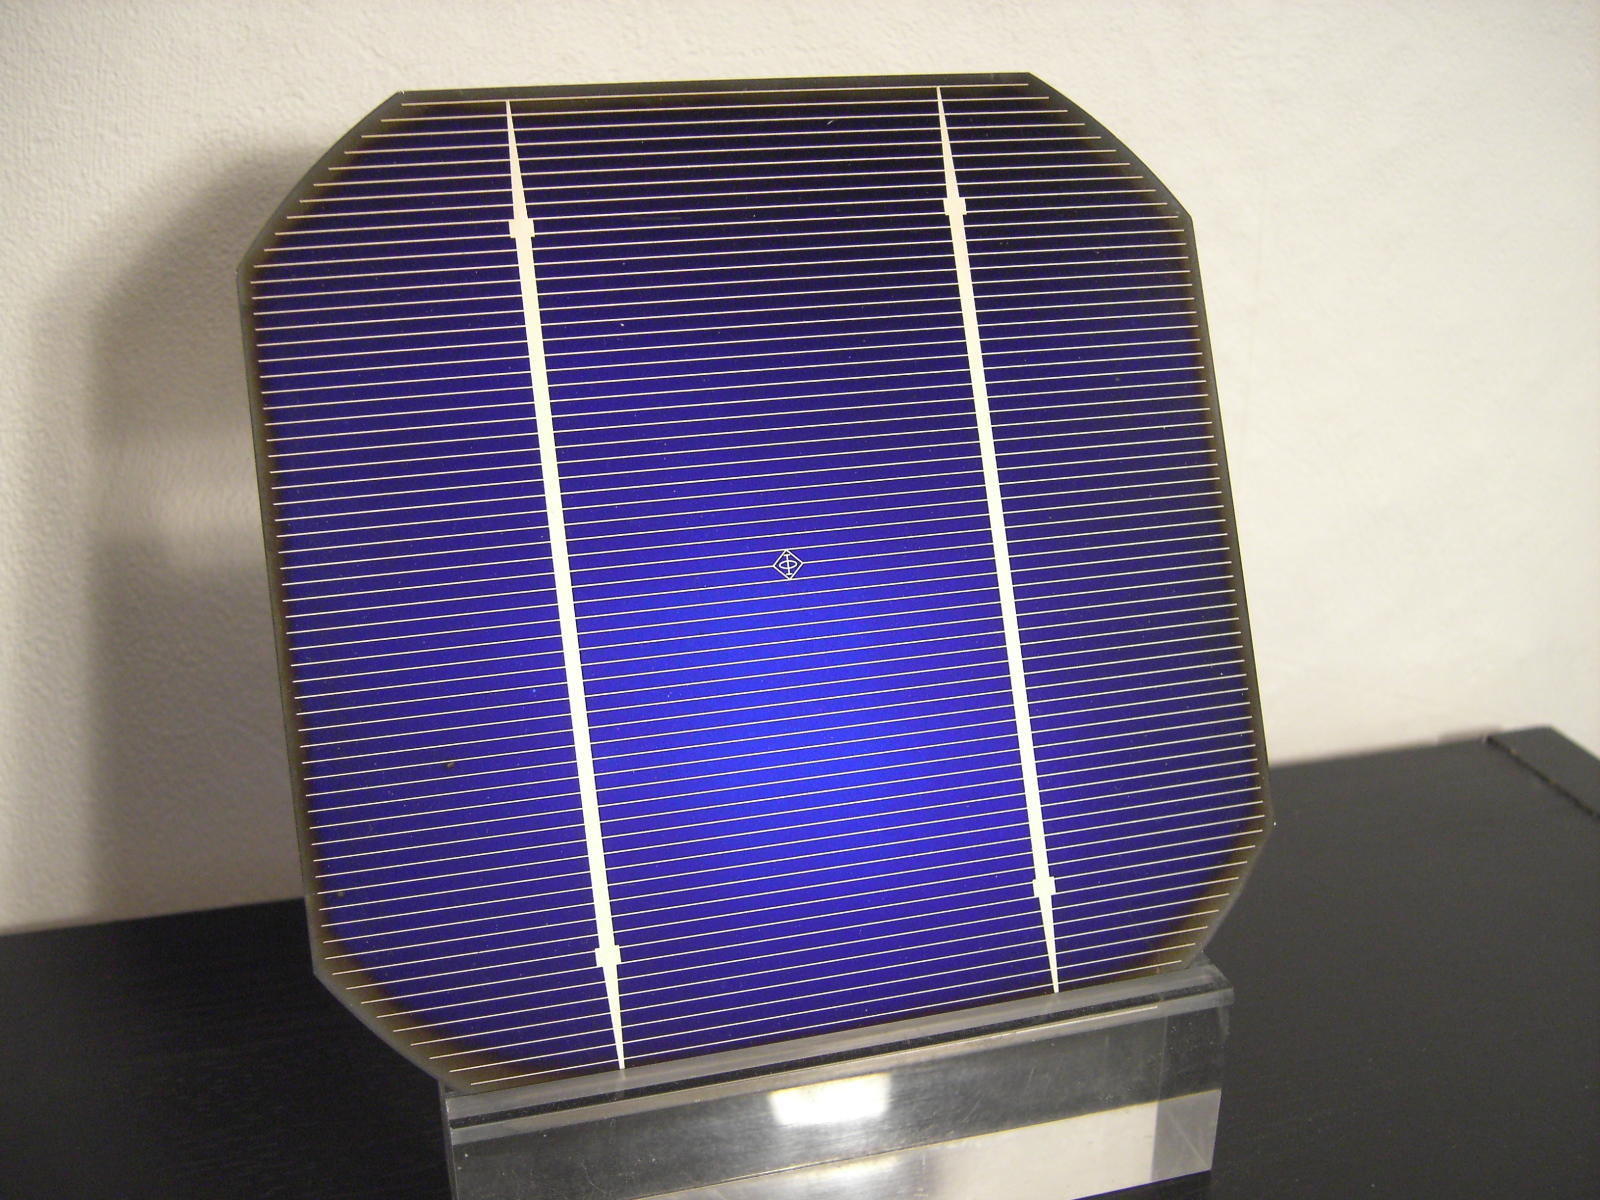
\includegraphics[width=350pt]{img/modulo-fotovoltaico.jpg}
\caption{Modulo fotovoltaico in silicio \emph{monocristallino}}
\end{figure}
%
Allo stato attuale, esistono diverse tecnologie di realizzazione di 
moduli fotovoltaici, la maggior parte delle quali basate su processi 
al silicio.
%

%
Per ogni modello di modulo fotovoltaico, le aziende 
costruttrici forniscono un \emph{datasheet}, riportanti i 
\emph{dati di targa} del modulo.
%
Tra i dati di targa, particolare importanza rivestono le curve 
\emph{corrente-tensione}, le quali caratterizzano l'andamento della tensione 
e della corrente - e, quindi, della potenza generata - ai capi del modulo, al 
variare di determinate \emph{grandezze d'influenza}.
%
Le curve corrente-tensione vengono tipicamente costruite mediante misurazioni
effettuate sotto \emph{standard test conditions} (STC)\cite{testconditions}, 
come indicato in tabella \ref{stc}, e variando di volta in volta una delle 
grandezze di influenza.
%
\begin{table}[htpb]
 \begin{center}
  \begin{tabular}{ | l | l | }
    \hline
    Radiazione & 1000 $W/m^2$ \\
    \hline
    Temperatura del modulo & 25  $\celsius$ \\
    \hline 
    Vento & 0 $m/s$ \\
    \hline
  \end{tabular}
  \caption{Condizioni di test standard (STC)}
  \label{stc}
 \end{center}
\end{table}
%

%
Un tipico esempio di curve corrente-tensione \`e mostrato in figura 
\ref{caratteristica_modulo_fv}: il primo dei due grafici mostra l'andamento 
della caratteristica al variare della radiazione solare, il secondo
invece mostra cosa accade al variare della temperatura superficiale del modulo.
%
\begin{figure}[!h]
\centering
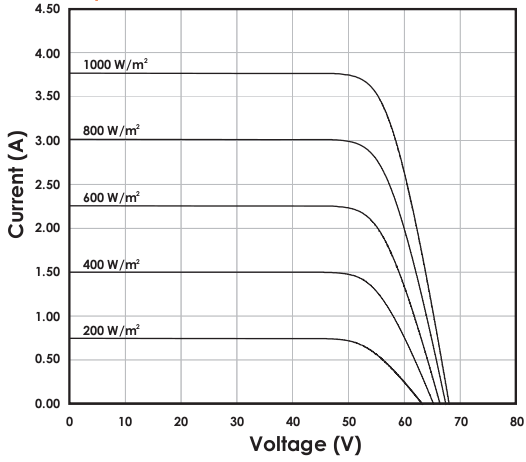
\includegraphics[width=190pt]{img/a-v-irradiance.png}
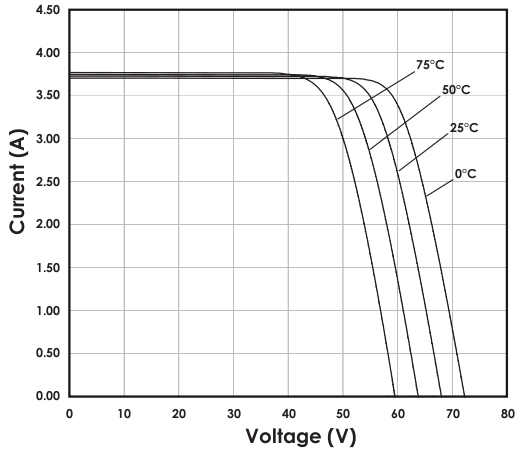
\includegraphics[width=190pt]{img/a-v-temperature.png}
\caption{Esempi di curve caratteristiche di un modulo fotovoltaico}
\label{caratteristica_modulo_fv}
\end{figure}
%% parlare della resistenza dei moduli e del decadimento delle prestazioni?
%

%
\subsection{Le stringhe fotovoltaiche}
Nei campi fotovoltaici, i singoli moduli sono tipicamente
raggruppati a formare delle \emph{stringhe}.
%
Per \emph{stringa fotovoltaica} si intende un insieme di moduli 
connessi in \emph{serie}. La connessione avviene mediante apposite 
\emph{junction box} generalmente collocate sul retro dei moduli.
%
\begin{figure}[!h]
\centering
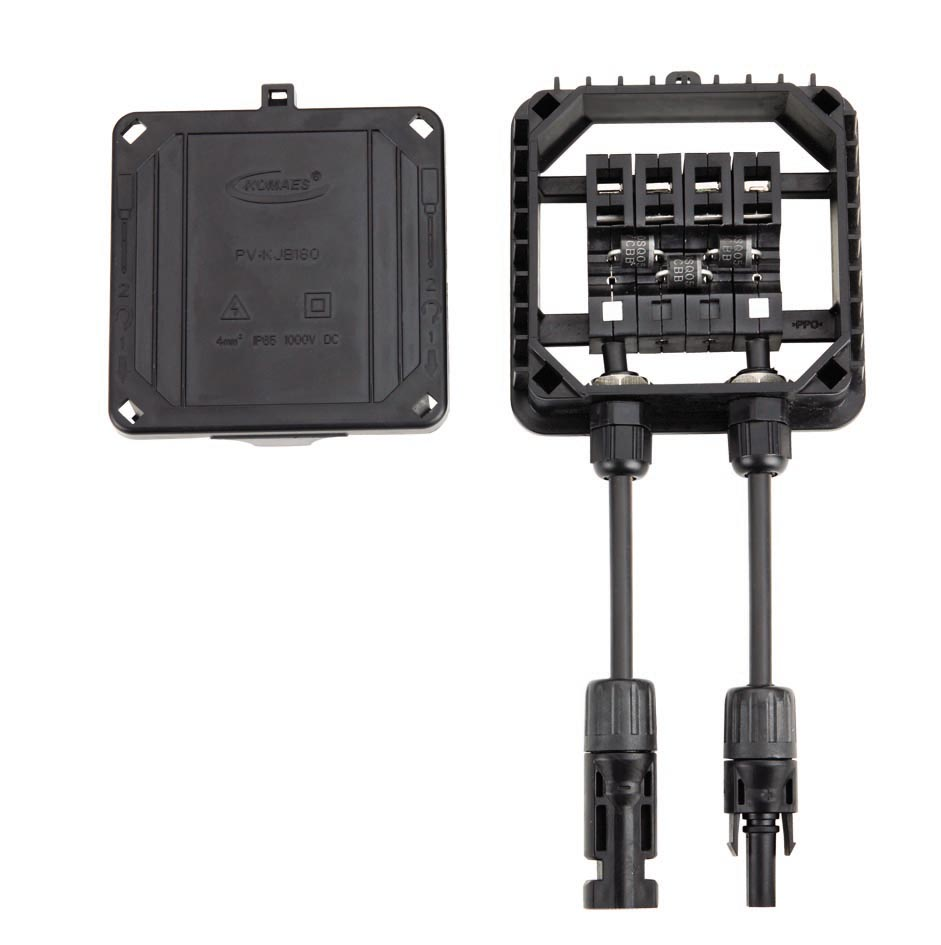
\includegraphics[width=190pt]{img/pv-junction-box.jpg}
\caption{Junction box}
\end{figure}
%
La connessione in serie implica che una eventuale differenza di 
performance tra moduli appartenenti alla stessa avr\`a come effetto 
un peggioramento di produzione per tutti i moduli della stringa.
%
Tale fenomeno, noto come \emph{mismatch di corrente}, pu\`o manifestarsi,
ad esempio, nel caso in cui uno o pi\`u moduli siano meno soleggiati 
di altri.













%% inverter
%% connessione alla rete









%% architettura tipica di un impianto fotovoltaico
%% quali informazioni si vogliono produrre?
%% quali informazioni e` necessario rilevare?
%% lista dei desiderata per un sistema di monitoraggio
